\subsubsection{Component overview}
\begin{figure}[h]
\centering
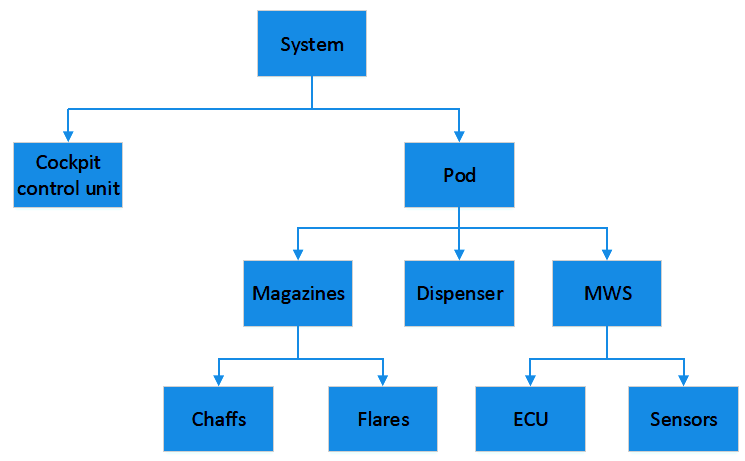
\includegraphics[scale=0.5]{./images/hierarchical.png}\\
\caption{Overview of components}
\label{fig:Component_overview}
\end{figure}

\begin{itemize}
\item Cockpit Control Unit (ID: CCU) 
\item Pod (ID: POD)
	\begin{itemize}
	\item Dispenser (ID: DIS)
	\item Magazines (ID: MAG)
	\end{itemize}
\end{itemize}
\begin{itemize}
\item MWS (ID: MWS)
	\begin{itemize}
	\item ECU (ID: ECU)
	\item Sensors (ID: SEN)
	\end{itemize}
\end{itemize}

\subsubsection{Detailed component description}
This section describes all system components and their connection to the requirements.

\paragraph{Cockpit Control Unit}\mbox{}\\
The Cockpit Control Unit (CCU) shall provide all necessary data to the aircraft mission computer.
\begin{itemize}
\item The CCU is responsible for switching between the three defined modes when receiving the respective signal from the aircraft mission computer (Req. No. 1-4 in F-SRS-2014-V1 ).
\item The CCU shall be able to turn power ON and OFF for the dispensing system and the MWS (Req. No. 7 in F-SRS-2014-V1 ).
\item The system shall be able to erase sensitive data upon input from a discrete zeroize signal from aircraft and the zeroize signal shall be received by the CCU (Req. No. 25-26 in F-SRS-2014-V1 ).
\item The system shall provide the aircraft mission computer with status information and built-in test results (Req. No. 15 in F-SRS-2014-V1 ).
\item The system status on individual LRU level shall be provided by cockpit unit (Req. No. 17 in F-SRS-2014-V1 ).
\end{itemize}

\paragraph{POD}\mbox{}\\
The pod is a detachable compartment on an aircraft for carrying chaffs and flares. The pod also holds the dispenser, magazines and the MWS.
\begin{itemize}
\item The pod structure must be functional when exposed to steady state acceleration levels of 4g forward, 2.5g backward, 22g upward or 10g downward.
\item The weight of the pod cannot exceed 270 kg (Req. No. 28 in F-SRS-2014-V1 ).
\item The pod shall be operational at temperatures of maximum 134 degree Celcius on outer skin and 152 degree Celcius on leading edge for maximum 3 minutes (Req. No. 29 in F-SRS-2014-V1 ).
\item The pod shall be operational at temperatures of maximum 95 degrees Celcius on outer skin and 152 degrees Celcius on leading egde for a maximum of 25 minutes (Req. No. 41 in F-SRS-2014-V1 ).
\item The physical dimensions of the pod cannot exceed 0.5$\times$0.5$\times$5 meter (Req. No. 35 in F-SRS-2014-V1 ).
\end{itemize}

\paragraph{Dispenser}\mbox{}\\
The dispenser is the mechanism in which the magazines are installed.
\begin{itemize}
\item The dispenser shall be able to dispense forwards, downwards and sideways (Req. No. 6 in F-SRS-2014-V1 ). 
\item The system shall be able to dispense a minimum of two payloads within 0.1 sec (Req. No. 8 in F-SRS-2014-V1 ).
\item The system shall be able to dispense a pattern of payloads programmable by the customer (Req. No. 9 in F-SRS-2014-V1 ).
\end{itemize}

\paragraph{Magazines}\mbox{}\\
The magazines contain the chaffs and flares.
\begin{itemize}
\item The pod shall include eight standard magazines (Req. No. 5 in F-SRS-2014-V1 ).
\item The magasines shall be stored at no lower than -10 degrees Celcius and no higher than 70 degrees Celcius (Req. No. 26 in F-SRS-2014-V1 ).
\end{itemize}

\paragraph{Chaffs and flares}\mbox{}\\
The chaffs and flares are the payload of the system. They are to be dispensed from the magazines.
\begin{itemize}
\item The aircraft has to be loaded with the payloads before takeoff (Req. No. 36 in F-SRS-2014-V1 ).
\end{itemize}

\paragraph{Missile Warning System}\mbox{}\\
The missile warning system (MWS) consists of an Electronic Control Unit and six sensors.
\begin{itemize}
\item The aircraft has to be loaded with the payloads before takeoff (Req. No. 36 in F-SRS-2014-V1 ).
\end{itemize}

\paragraph{Electronic Control Unit}\mbox{}\\
\begin{itemize}
\item The Electronic Control Unit (ECU) provides threat information in inertial format and the direction of the threat is relative to north (Req. No. 14 in F-SRS-2014-V1 ).
\end{itemize}

\paragraph{Sensors}\mbox{}\\
The sensors are responsible for detecting incoming missiles (threats).